\chapter{动物如何成长}\label{ch:g2:animals-grow-up}

小猫从出生第一天起，看上去就是一只小猫。但
池塘里的青蛙，最初是一只形似小鱼、没有腿的\omterm{ex:g2:animals-grow-up:frog}{蝌蚪}，
停在醉鱼草上的蝴蝶，曾有数周是一条爬行的
\omterm{ex:g2:animals-grow-up:butterfly}{毛毛虫}。幼年\omterm{def:g1:animals-around-us:animal}{动物}并不都与父母相像——
有些必须在长成成体的过程中彻底变形。

\section{从卵孵化还是胎生}

\begin{definition}[两种出生方式]\label{def:g2:animals-grow-up:born}
幼年\omterm{def:g1:animals-around-us:animal}{动物}来到世上有两种方式：
\begin{itemize}
  \item 大多数是由母亲产下的\emph{卵}\index{卵}孵化而来：
        鸟类、鱼类、青蛙、蜗牛和昆虫；
  \item 其他\omterm{def:g1:animals-around-us:animal}{动物}是\emph{胎生出生}\index{胎生出生}，
        已发育成形，从母体中产出，并吸食母亲的
        \emph{乳汁}\index{乳汁}：猫、狗、牛、兔子——还有
        人类。
\end{itemize}
\end{definition}

\begin{example}[鸡舍与篮子]\label{ex:g2:animals-grow-up:henhouse}
母鸡下蛋，并趴在蛋上保温；三
周后，小鸡啄破蛋壳孵化。炉子旁的
篮子里，猫妈妈的小猫们当晚出生，
并在一小时之内就找到了母猫的\omterm{def:g2:animals-grow-up:born}{乳汁}。
\end{example}

\begin{remark}[卵不是石头]\label{rem:g2:animals-grow-up:egg}
被母鸡孵着的卵里，小鸡正在悄悄地长成，
靠黄色的卵黄提供养分。卵并不是在等待，而是在工作。这就是母鸡要让卵保持温暖的原因，
也是为什么从冰箱里拿出的卵，
本就不会孵化，也不能怪到寒冷头上。
\end{remark}

\section{不变形的成长}

\begin{definition}[像父母一样成长]\label{def:g2:animals-grow-up:direct}
许多幼年\omterm{def:g1:animals-around-us:animal}{动物}都是\emph{父母的
缩小版}\index{父母的缩小版}：小猫是一只小
猫，小马驹是一匹小马，小鸡是一只小母鸡。长大
对它们来说，长大意味着变得更大、更强壮——身体的形状
始终不变。
\end{definition}

\begin{example}[从小猫到成猫]\label{ex:g2:animals-grow-up:kitten}
刚出生的小猫闭着眼睛吮吸\omterm{def:g2:animals-grow-up:born}{乳汁}。一个月时，它
会玩耍、会扑跳；六个月时，它像成年猫一样捕猎；
满一年时，它已是成年猫，也许还有了自己的小猫。
小猫、大猫、成猫：一路上形态始终不变。
\end{example}

\section{通过变态成长}

\begin{definition}[变态]\label{def:g2:animals-grow-up:metamorphosis}
有些幼年\omterm{def:g1:animals-around-us:animal}{动物}与父母毫不相像，必须
改变全身的形态，才能成为成体。这一巨大的变化
称为\emph{变态}\index{变态}。\omterm{ex:g2:animals-grow-up:frog}{蝌蚪}
变成青蛙；\omterm{ex:g2:animals-grow-up:butterfly}{毛毛虫}变成蝴蝶。
\end{definition}

\begin{example}[青蛙的成长之路]\label{ex:g2:animals-grow-up:frog}
池塘里青蛙的卵孵出\emph{蝌蚪}\index{蝌蚪}：
头圆、尾长、无腿，像鱼一样在水中呼吸。
接着，一周接一周：后腿长出，然后是前腿；尾巴
逐渐缩小；有一天，一只小青蛙爬上了岸。
同一个\omterm{def:g1:animals-around-us:animal}{动物}——只是重新塑造了一番。
\end{example}

\begin{omfigure}
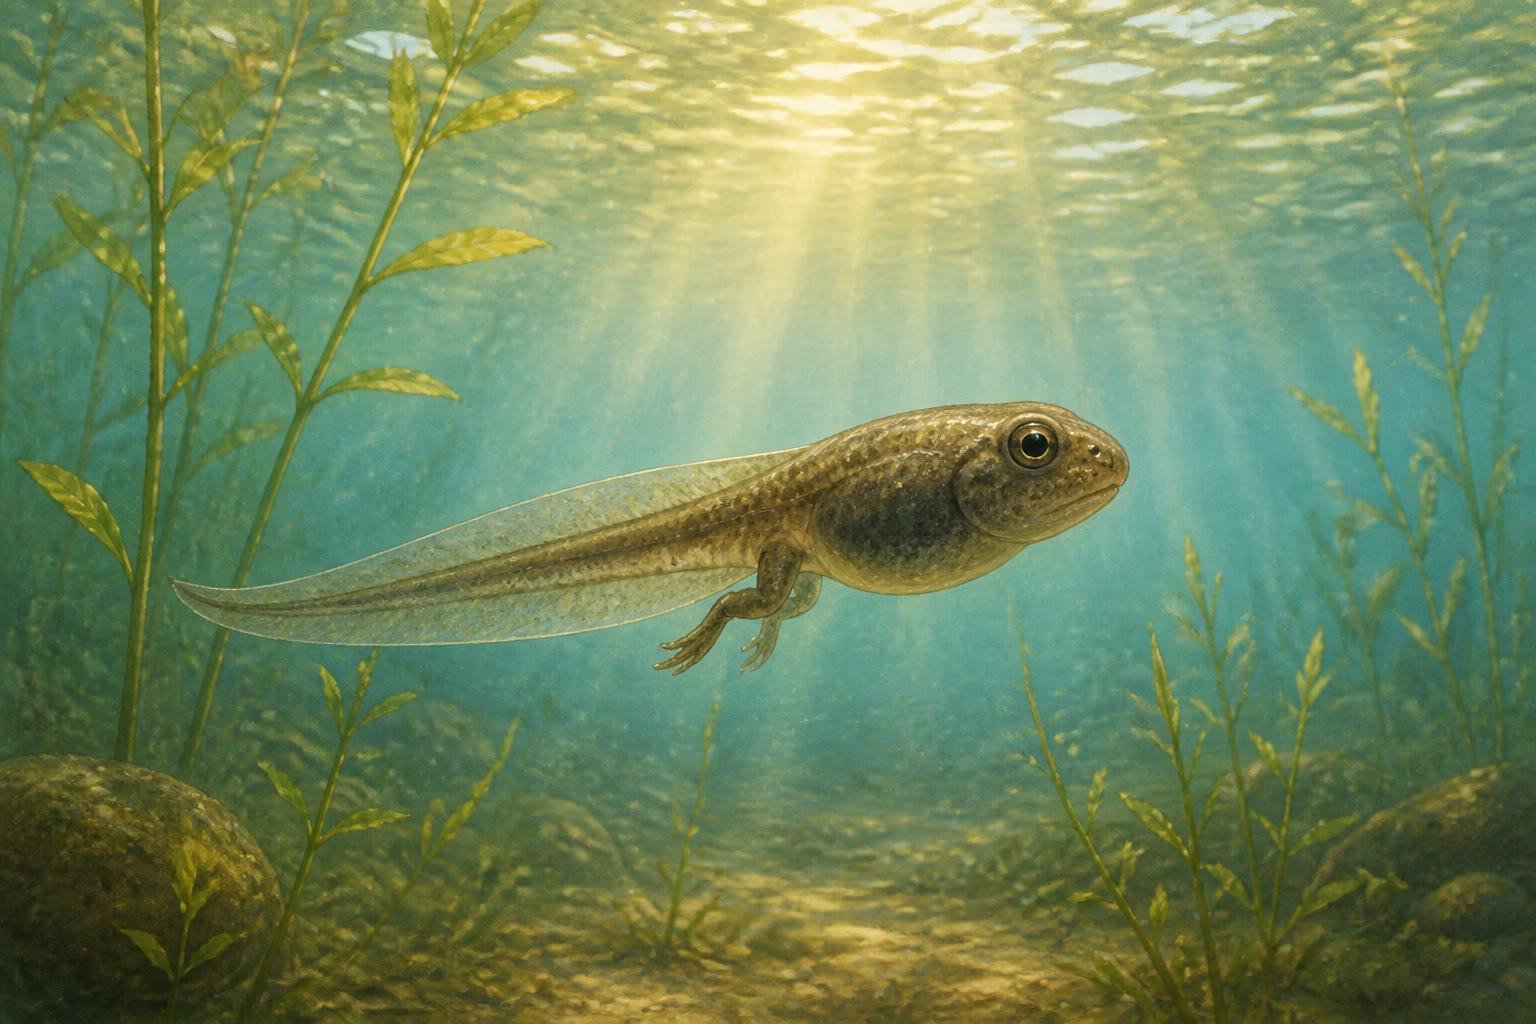
\includegraphics[width=0.6\linewidth]{images/book1/ai/g2-grow-tadpole.jpg}

{\small \omterm{def:g2:animals-grow-up:metamorphosis}{变态}途中抓拍：后腿已长出，前腿
尚未长出，尾巴仍然很长。}
\end{omfigure}

\begin{omfigure}
\begin{tikzpicture}
  \node[anchor=south west, inner sep=0] (img) at (0,0)
    {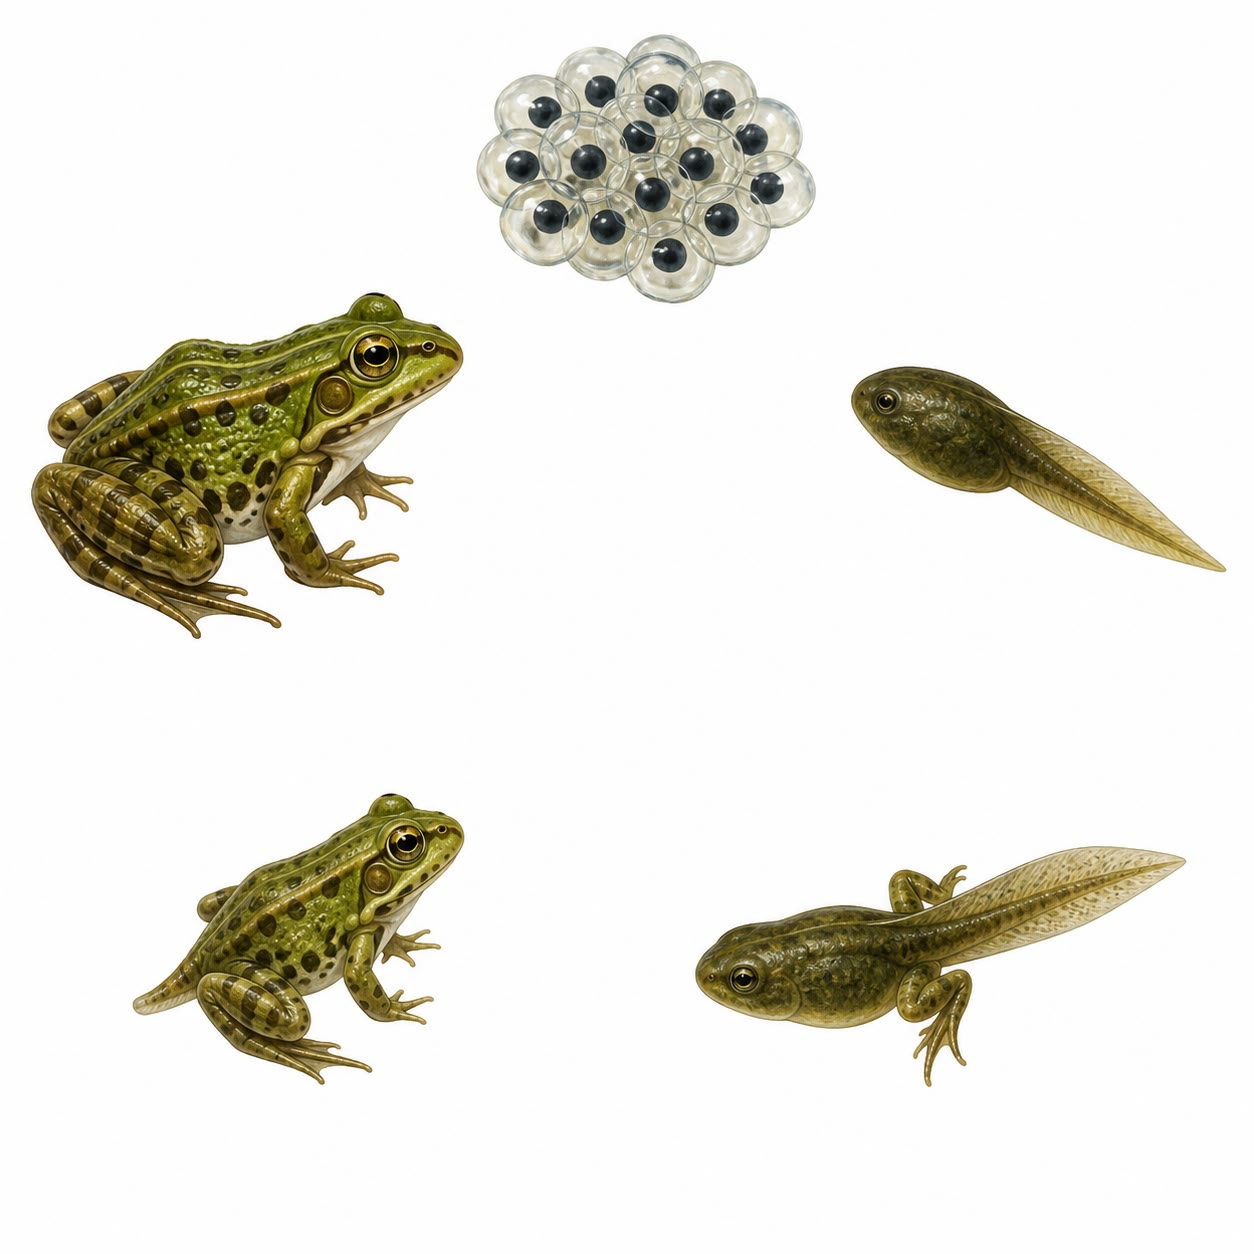
\includegraphics[width=0.72\linewidth]{images/book1/ai/fig-frog-cycle.jpg}};
  \begin{scope}[x={(img.south east)}, y={(img.north west)},
      every node/.style={font=\small}]
    \node[above] at (0.33,0.92) {池塘中的卵};
    \node[right, align=left] at (0.87,0.44)
      {蝌蚪：\\ 有尾巴，无腿};
    \node[below, align=center] at (0.80,0.05)
      {后腿长出，\\ 然后前腿长出};
    \node[below] at (0.22,0.05) {尾巴缩小：幼蛙};
    \node[left, align=right] at (0.075,0.78) {成年青蛙};
    \draw[->, thick, omProp] (0.70,0.86) to[bend left=20] (0.87,0.68);
    \draw[->, thick, omProp] (0.88,0.38) to[bend left=15] (0.85,0.25);
    \draw[->, thick, omProp] (0.60,0.16) to[bend left=12] (0.42,0.14);
    \draw[->, thick, omProp] (0.16,0.32) to[bend left=15] (0.13,0.48);
    \draw[->, thick, omProp] (0.30,0.80) to[bend left=18] (0.42,0.88);
  \end{scope}
\end{tikzpicture}

{\small 青蛙的\omterm{def:g2:animals-grow-up:metamorphosis}{变态}过程，从卵开始按顺时针方向看：
卵、\omterm{ex:g2:animals-grow-up:frog}{蝌蚪}、长腿、幼蛙、成体——成体又会
产下新的卵。}
\end{omfigure}

\begin{example}[蝴蝶的成长之路]\label{ex:g2:animals-grow-up:butterfly}
蝴蝶的卵孵出\emph{毛毛虫}\index{毛毛虫}，
它几乎只是吃\omterm{def:g1:plants-around-us:parts}{叶子}、长大。有一天，它把自己
裹进一个外壳，即\emph{蛹}\index{蛹}，然后停止活动。
在壳内，身体被重新塑造；几周后，外壳裂开，
一只蝴蝶爬了出来，展开湿润的新翅膀。卵、\omterm{ex:g2:animals-grow-up:butterfly}{毛毛虫}、
蛹、蝴蝶：同一个\omterm{def:g1:animals-around-us:animal}{动物}的四个阶段。
\end{example}

\begin{method}[读懂动物的生命周期]\label{met:g2:animals-grow-up:read}
遇到任何\omterm{def:g1:animals-around-us:animal}{动物}，可以依次思考：
\begin{enumerate}
  \item 问一问它是怎样出生的：从卵里孵出，还是直接活着生下来？
  \item 问一问幼体长什么样：是\omterm{def:g2:animals-grow-up:direct}{父母的缩小版}，
        还是另一种模样？
  \item 如果模样不同，它就会\omterm{def:g2:animals-grow-up:metamorphosis}{变态}：找一找
        它\omterm{def:g2:animals-grow-up:metamorphosis}{变态}过程中的各个阶段；
  \item 把\omterm{def:g2:born-grow-die:cycle}{生命周期}画成一个圆圈，从成体
        画一个箭头指回卵。
\end{enumerate}
\end{method}

\begin{remark}[奶水，还是直接自立]\label{rem:g2:animals-grow-up:care}
小猫几周内都由妈妈喂养、清洁；刚
孵出的\omterm{ex:g2:animals-grow-up:frog}{蝌蚪}得不到任何帮助，从第一天起就得自己觅食。
有些幼体受到照料，另一些则
独自开始生活——两条路都通向成年。
\end{remark}

\section{练习}

\begin{exercise}[$\star$]\label{exo:g2:animals-grow-up:1}
说出幼体来到世界的两种方式，
每种各举一个例子。
\end{exercise}

\begin{exercise}[$\star$]\label{exo:g2:animals-grow-up:2}
判断下列\omterm{def:g1:animals-around-us:animal}{动物}是从卵里孵出，还是直接活着生下：（a）小鸡；（b）小猫；（c）
青蛙；（d）兔子；（e）蜗牛？
\end{exercise}

\begin{exercise}[$\star$]\label{exo:g2:animals-grow-up:3}
小猫出生后最先喝的是什么？本章中的哪些\omterm{def:g1:animals-around-us:animal}{动物}
出生时也喝同样的东西？
\end{exercise}

\begin{exercise}[$\star$]\label{exo:g2:animals-grow-up:4}
什么是\omterm{def:g2:animals-grow-up:metamorphosis}{变态}？
请说出本章中两个著名的例子。
\end{exercise}

\begin{exercise}[$\star$]\label{exo:g2:animals-grow-up:5}
把青蛙的各阶段排好顺序：青蛙——卵——长出
后腿的\omterm{ex:g2:animals-grow-up:frog}{蝌蚪}——\omterm{ex:g2:animals-grow-up:frog}{蝌蚪}。
\end{exercise}

\begin{exercise}[$\star$]\label{exo:g2:animals-grow-up:6}
把蝴蝶的各阶段排好顺序：蝴蝶——\omterm{ex:g2:animals-grow-up:butterfly}{毛毛虫}——
卵——蛹。哪个阶段的\omterm{def:g1:animals-around-us:animal}{动物}吃\omterm{def:g1:plants-around-us:parts}{叶子}、
长得最快？
\end{exercise}

\begin{exercise}[$\star$]\label{exo:g2:animals-grow-up:7}
哪一种幼体是\omterm{def:g2:animals-grow-up:direct}{父母的缩小版}：\omterm{ex:g2:animals-grow-up:frog}{蝌蚪}，还是
小马驹？对于这种幼体来说，长大意味着什么？
\end{exercise}

\begin{exercise}[$\star$]\label{exo:g2:animals-grow-up:8}
母鸡为什么要趴在卵上？卵里正在发生什么，
由\cref{rem:g2:animals-grow-up:egg}可知？
\end{exercise}

\begin{exercise}[$\star\star$]\label{exo:g2:animals-grow-up:9}
在池塘里，佐伊发现一只小\omterm{def:g1:animals-around-us:animal}{动物}：头是圆的，
尾巴长长的，有两条后腿，没有前腿。请对照青蛙的\omterm{def:g2:born-grow-die:cycle}{生命周期}图，
说出它正处在哪个阶段，它之前是什么样子，
以及接下来会变成什么。
\end{exercise}

\begin{exercise}[$\star\star$]\label{exo:g2:animals-grow-up:10}
“\omterm{ex:g2:animals-grow-up:butterfly}{毛毛虫}在外壳里死去了，一只蝴蝶搬了进来。”
蛹里面究竟发生了什么？请结合
\cref{def:g2:animals-grow-up:metamorphosis}和
\cref{ex:g2:animals-grow-up:butterfly}作答。
\end{exercise}
